% !TEX root = /home/computer/ucsc/master-2/quarter-2/numerical-linear-algebra/master.tex
\assignment{2}{Wed 02 Feb 2022 20:27}{Assignment 2}

\subsectionfont{\fontsize{10}{10}\selectfont}

% \usepackage{alltt}


\graphicspath{{./assignment_02/figures/}}

\section{Part 1}%
\label{sec:part_1}

\subsection{Output for Trace, Gaussian Elimination, LU decomposition and Two
norm of Error in solution to AX = B}%

\verbatiminput{{./assignment_02/code/output.txt}}

\subsection{Plane Equation}%
\label{sub:plane_equation}

The equation of a plane can be solved for $a, b, c, d$ using the points
$ A(1,2,3)$, $ B(-3, 2, 5)$, and $ C(\pi, e, - \sqrt{2})$, by solving the
following equation for 

\begin{align*}
  a + 2b + 3c + d &= 0 \\
  -3a + 2b + 5c + d &= 0 \\
  \pi a + e b - \sqrt{2}c + d &= 0
\end{align*}

\verbatiminput{{./assignment_02/code/plane.txt}}

\begin{figure}[H]
  \centering
  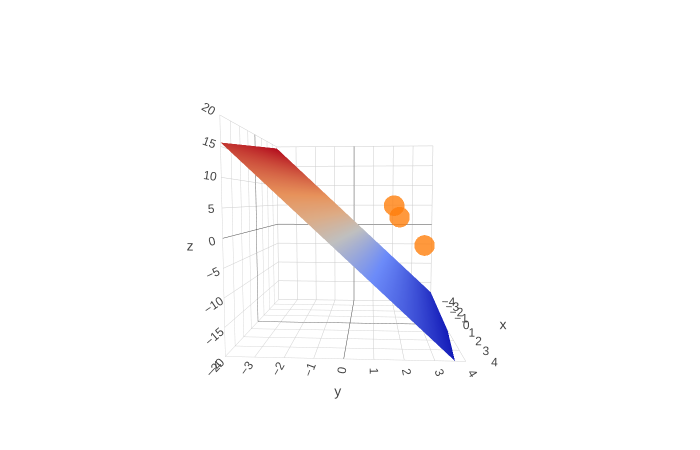
\includegraphics[width=0.8\linewidth]{newplot_.png}
\end{figure}

\section{Part 2}%
\label{sec:part_2}

\subsection{Schur decomposition of a symmetric matrix}%
\label{sub:schur_decomposition_of_a_symmetric_matrix}

If $A \in \C^{m\times m}$, then there exists a unitary matrix $Q$ and an upper
triangular matrix $U$ such that $A = QUQ^{*}$. 

If $A$ is (real) symmetric then

\[
   A = QUQ^{T} = QU^{T}Q^{T} = A^{T}
.\] 

This implies
\[
U = U^{T}
.\] 

and the only way this can happen is if $U = D$ is diagonal, so the Schur
decomposition implies that $A$ is orthogonally diagonalizable
\[
A = QDQ^{T}
.\] 

where the columns of $Q$ form an eigenbasis for $A$, and  $Q^{T}$ is the change
of basis matrix that transforms $A$ into a diagonal matrix $D$ of eigenvalues
of $A$.

\subsection{Stability of Gaussian elimination}%
\label{sub:stability_of_gaussian_elimination}

Consider
\[
\begin{pmatrix}
  1 & 1 \\ \epsilon & 1
\end{pmatrix} \begin{pmatrix}
  x \\ y
\end{pmatrix} = \begin{pmatrix}
  2 \\ 1
\end{pmatrix}
.\] 

Multiply the last row by $c$ so that $c \epsilon \gg 1$, then swapping row one with
row two. The augmented system becomes
\[
  \begin{pmatrix}
    c \epsilon & c & c \\
    1 & 1 & 2
  \end{pmatrix}
.\] 

the elimination step
\[
\begin{pmatrix}
  c \epsilon & c & c \\
  0 & 1-\frac{1}{\epsilon }  & 2-\frac{1}{\epsilon }
\end{pmatrix}
.\] 

which is numerically equivalent to
\[
\begin{pmatrix}
  c \epsilon & c & c \\
  0 & -\epsilon ^{-1} & \epsilon ^{-1}
\end{pmatrix}
.\] 

and leads to the incorrect solution
\[
  y = \frac{-\epsilon ^{-1}}{-\epsilon ^{-1}} = 1 \qquad
  x = \frac{1-1}{\epsilon } = 0
.\] 

The issue partial pivoting hoped to correct was reintroduced by scaling the row
with a smaller pivot. 

\subsection{Diagonal entries of a symmetric positive definite matrix}%
\label{sub:diagonal_entries_of_a_symmetric_positive_definite_matrix}

If $A$ is symmetric positive definite then for all $v$
\[
v^{T}Av > 0
.\] 

Considering the standard basis vectors $e_{j}$ 

\[
e_{j}^{T}Ae_{j} = a_{jj}
.\] 

Since any vector $v$ can be written as a linear
combination of these basis vectors
\[
v = v_1e_1 + \dots + v_{n}e_{n}
.\] 

then
\[
  v^{T}Av = \sum^{n}_{j=1} a_{jj}v_{j}^{2} > 0
.\] 

implies $a_{jj} > 0$

\subsection{LU decomposition of a block matrix}%
\label{sub:lu_decomposition_of_a_block_matrix}
\subsubsection{Verify the formula}%
\label{ssub:part_a}

\begin{align*}
  \begin{pmatrix} I & 0 \\ -A_{21}A_{11}^{-1} & I \end{pmatrix} \begin{pmatrix} A_{11} & A_{12} \\ A_{21} & A_{22} \end{pmatrix} &= \begin{pmatrix} A_{11} & A_{12} \\ -A_{21}A_{11}^{-1}A_{11} + A_{21} & -A_{21}A_{11}^{-1}A_{12} + A_{22} \end{pmatrix} \nonumber \\
  &= \begin{pmatrix} A_{11} & A_{12} \\ 0 & A_{22}-A_{21}A_{11}^{-1}A_{12} \end{pmatrix} \\
\end{align*}

\subsubsection{Show ${\bf D =A_{22}-A_{21}A_{11}^{-1}A_{12}}$ after ${\bf n}$
steps of Gaussian elimination }%
\label{ssub:part_b}

\[
\begin{pmatrix}
  A_{11} & A_{12} \\ A_{21} & A_{22}    
\end{pmatrix} \implies  \begin{pmatrix}
  A_{11} & C \\
  0 & D
\end{pmatrix}
.\] 


    First defining the matrix $R_{i}$ as the matrix that contains the negation
    of the $i^{\text{th}}$ row of $A_{21}$ and zeros everywhere else. Then
    performing $n$ steps of Gaussian elimination on $A$ using block elementary
    matrices
    \[
    E_{i} = \begin{pmatrix}
      I & 0 \\
      R_{i}A_{11}^{-1} & I
    \end{pmatrix}
    .\] 

    eliminates the block matrix $A_{21}$ 
    \begin{align*}
      E_{n} \dots E_1 A &= \begin{pmatrix}
        I & 0 \\
        R_{n}A_{11}^{-1} & I
      \end{pmatrix} \dots \begin{pmatrix}
        I & 0 \\
        R_{1}A_{11}^{-1} & I
      \end{pmatrix} \begin{pmatrix}
        A_{11} & A_{12} \\
        A_{21} & A_{22}
      \end{pmatrix}
                        &= \begin{pmatrix}
                          A_{11} & C \\
                          0 & D
                        \end{pmatrix}
    \end{align*}

    where 
    \begin{align*}
      E_{n} \dots E_1 &= \begin{pmatrix}
        I & 0 \\
        R_{n}A_{11}^{-1} & I
      \end{pmatrix} \dots \begin{pmatrix}
        I & 0 \\
        R_{1}A_{11}^{-1} & I
      \end{pmatrix} \\
                      &= \begin{pmatrix}
                        I & 0 \\
                        R_{n}A_{11}^{-1} + \dots + R_{1}A_{11}^{-1} & I
                      \end{pmatrix} \\
                      &= \begin{pmatrix}
                        I & 0 \\
                        (R_{n} + \dots + R_{1})A_{11}^{-1} & I
                      \end{pmatrix} \\
                      &= \begin{pmatrix}
                        I & 0 \\ -A_{21}A_{11}^{-1} & I
                      \end{pmatrix}
    \end{align*}

    which is exactly what we used to verify the formula in $(\ref{ssub:part_a})$

\subsection{${\bf Ax = b}$ complex valued}%
\label{sub:_bf_ax_b_complex_valued}

\subsubsection{Modify problem}%
\label{ssub:modify_problem}

Decompose $A = A_{1} + iA_2$ and $b = b_1 + ib_2$ then
\begin{gather*}
  Ax = b \\
  (A_1 + iA_2)x = b_1 + i b_2
\end{gather*}

equating the real and imaginary parts this is equivalent to solving 
\[
A_1x_1 = b_1 \qquad A_2x_2 = b_2
.\] 

where $x_1 = \text{Re} (x)$,  $x_2 = \text{Im} (x)$, and both systems are real

\subsubsection{Compare storage and number of floating point operations}%
\label{ssub:compare_storage_and_number_of_floating_point_operations}

Consider complex numbers $ a_{ij}/a_{jj} $ used in Gaussian elimination

\[
  \frac{a_{ij}}{a_{jj}} = \frac{(a,b)}{ (c,d) } = \frac{ (ac +bd, -ad
  +bc)}{c^2+d^2}
.\] 

this introduces $6$ multiplications and $3$ additions, compared to just $1$
operation if they were real. The storage requirements for the complex case $Ax
= b$ is the same as for the two systems $A_1x_1 = b_1$ and $A_2x_2 = b_2$.


% \begin{minted}{julia}
% do j = 1: m-1
%   do i = j+1: m
%     ri = ri - rj*(aij/ajj)
% \end{minted}
